\documentclass[a4paper,12pt]{article}

\usepackage[T2A]{fontenc}			
\usepackage[utf8]{inputenc}			
\usepackage[english,russian]{babel}	

\usepackage[
bookmarks=true, colorlinks=true, unicode=true,
urlcolor=black,linkcolor=black, anchorcolor=black,
citecolor=black, menucolor=black, filecolor=black,
]{hyperref}

\usepackage{color}
\usepackage{caption}
\DeclareCaptionFont{white}{\color{black}}
\DeclareCaptionFormat{listing}{\colorbox{white}{\parbox{\textwidth}{#1#2#3}}}
\captionsetup[lstlisting]{format=listing,labelfont=white,textfont=white}

\usepackage{amsmath,amsfonts,amssymb,amsthm,mathtools} 
\usepackage{wasysym}

\usepackage{graphicx}
%\usepackage[cache=false]{minted}
\usepackage{cmap}
\usepackage{indentfirst}

\usepackage{listings} 
\usepackage{fancyvrb}

\usepackage{geometry}
\geometry{left=2cm}
\geometry{right=1.5cm}
\geometry{top=1cm}
\geometry{bottom=2cm}

\setlength{\parindent}{5ex}
\setlength{\parskip}{0.5em}

\usepackage{pgfplots}

\usepackage{longtable}

\begin{document}
	\lstset{ %
		language=C,                 % выбор языка для подсветки (здесь это С)
		basicstyle=\small\sffamily, % размер и начертание шрифта для подсветки кода
		numbers=left,               % где поставить нумерацию строк (слева\справа)
		numberstyle=\tiny,           % размер шрифта для номеров строк
		stepnumber=1,                   % размер шага между двумя номерами строк
		numbersep=5pt,                % как далеко отстоят номера строк от подсвечиваемого кода
		backgroundcolor=\color{white}, % цвет фона подсветки - используем \usepackage{color}
		showspaces=false,            % показывать или нет пробелы специальными отступами
		showstringspaces=false,      % показывать или нет пробелы в строках
		showtabs=false,             % показывать или нет табуляцию в строках
		frame=single,              % рисовать рамку вокруг кода
		tabsize=2,                 % размер табуляции по умолчанию равен 2 пробелам
		captionpos=t,              % позиция заголовка вверху [t] или внизу [b] 
		breaklines=true,           % автоматически переносить строки (да\нет)
		breakatwhitespace=false, % переносить строки только если есть пробел
		escapeinside={\%*}{*)}   % если нужно добавить комментарии в коде
	}
	
	% Титульный лист
	\begin{figure}[h!]
		\begin{center}
			{
\includegraphics[scale = 0.4]{titul.jpg}}
			\label{titul}
		\end{center}
	\end{figure}
	
	\vspace*{15mm} 
	
	\huge
	\begin{center}
		Дисциплина: <<Моделирование>>
	\end{center}
	
	\begin{center}
		Лабораторная работа №5
	\end{center}

	
	\huge
	\begin{center}
		Тема работы:\\
		<<Моделирование информационного центра>>
	\end{center}
	\vspace*{25mm} 
	
	\large
	\begin{flushright}
		Студент: Левушкин И. К. \\
		Группа: ИУ7-72Б \\
		Преподаватель: Рудаков И. В. \\
	\end{flushright}
	
	\vspace*{25mm}
	\begin{center}
		Москва, 2020 г.  
	\end{center}
	\thispagestyle{empty}
	
	
	\newpage
	
	\section*{Задание}
	
	В информационный центр приходят клиенты через интервал времени $10 \pm 2$ минуты. Если все три имеющихся оператора заняты, клиенту отказывают в обслуживании. Операторы имеют разную производительность и могут обеспечивать обслуживание среднего запроса пользователя за $20 \pm 5$; $40 \pm 10$; $40 \pm 20$. Клиенты стремятся занять свободного оператора с максимальной производительностью. Полученные запросы сдаются в накопитель. Откуда выбираются на обработку. На первый компьютер запросы от 1 и 2-ого операторов, на второй – запросы от 3-его. Время обработки запросов первым и 2-м компьютером равны соответственно 15 и 30 мин. Промоделировать процесс обработки 300 запросов. 
	Необходимо для этого создать концептуальную модель в терминах СМО, определить эндогенные и экзогенные переменные и уравнения модели.
	
	\newpage
	
	\section*{Формализация}
	
	\subsection*{Концептуальная модель}
	
	Ниже приведена концептуальная модель и концептуальная модель в терминах СМО.
	
	\begin{figure}[h!]
		\begin{center}
			{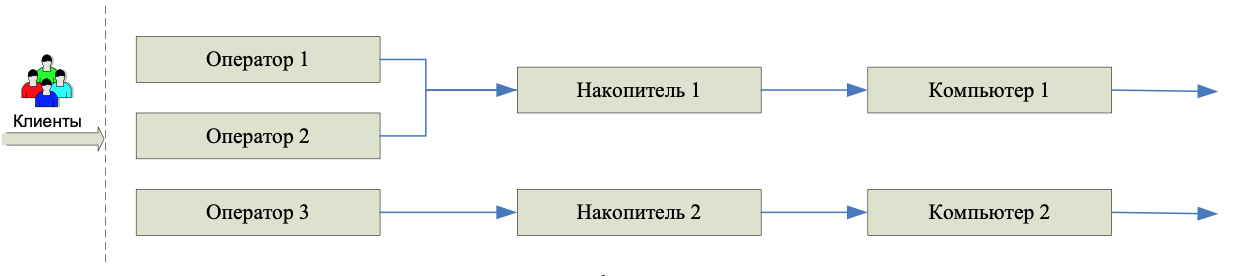
\includegraphics[scale = 0.6]{model1.png}}
			\label{ris:model1}
		\end{center}
		\caption{Концептуальная модель.}
	\end{figure}

	\begin{figure}[h!]
		\begin{center}
			{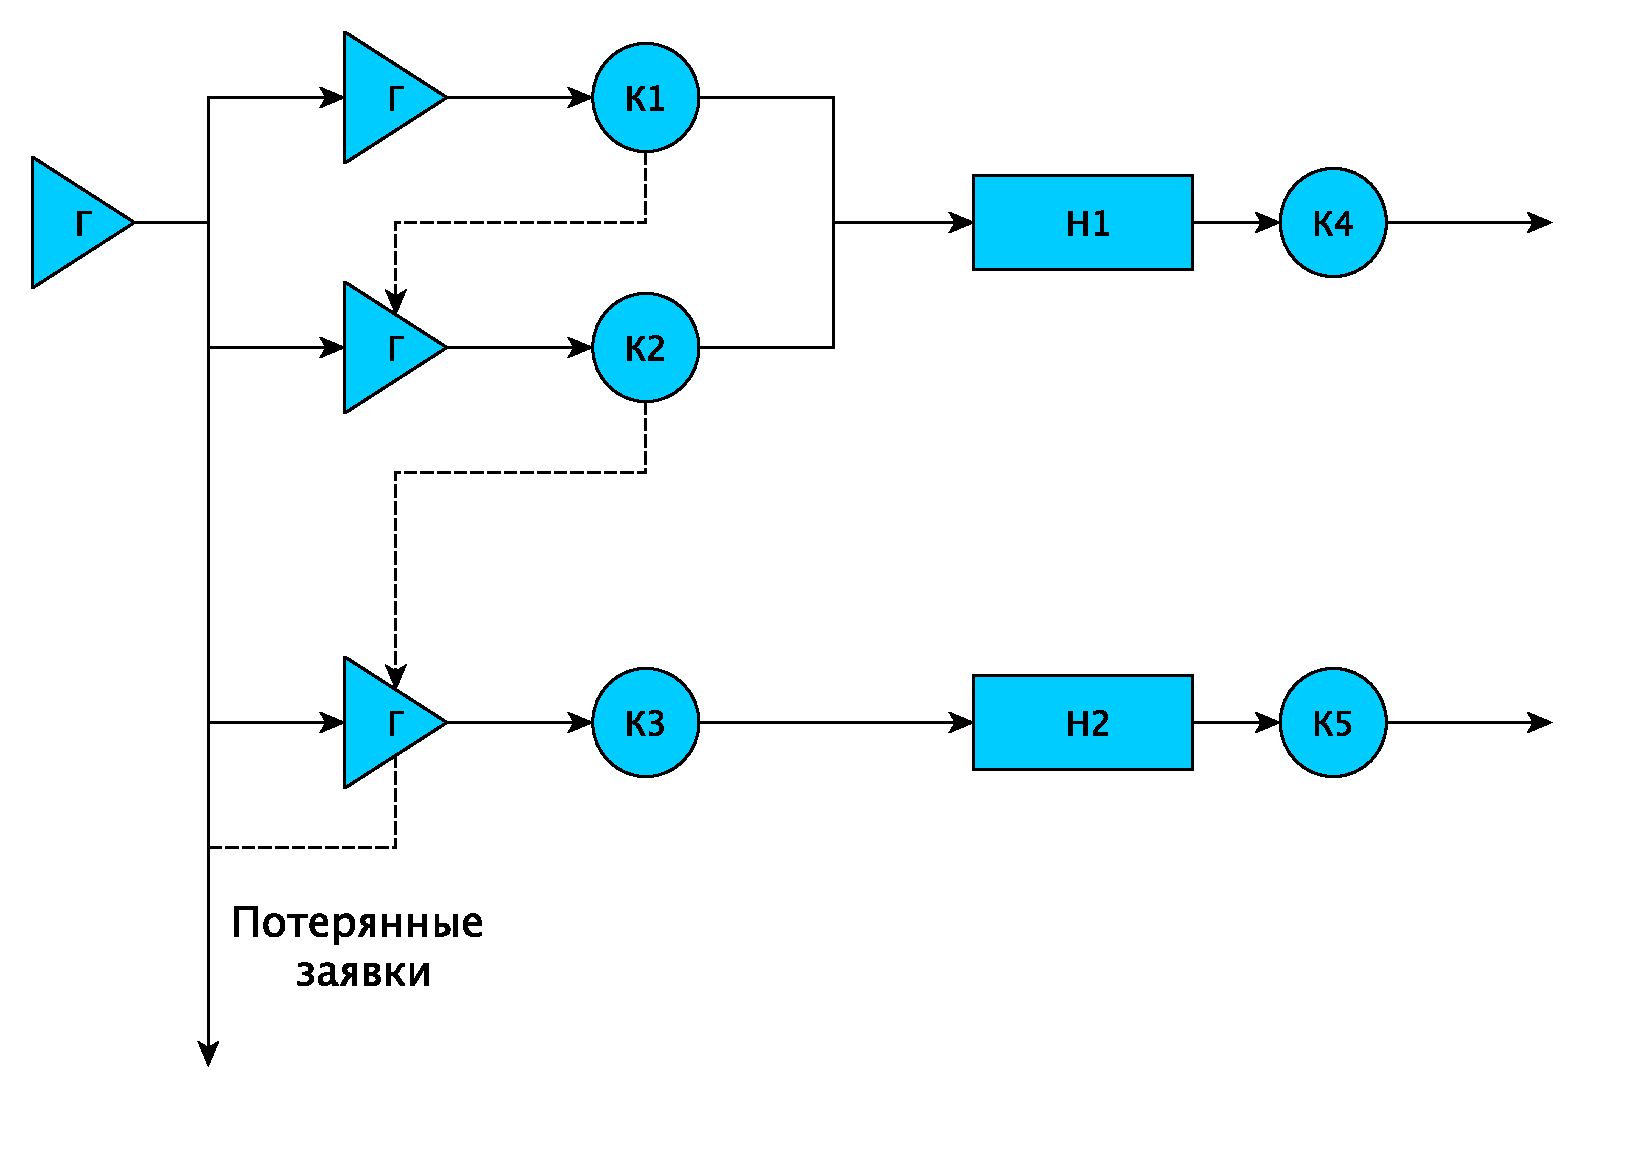
\includegraphics[scale = 0.6]{model2.pdf}}
			\label{ris:model2}
		\end{center}
		\caption{Концептуальная модель в терминах СМО.}
	\end{figure}
	
	В процессе взаимодействия клиентов с информационным центром возможно:
	\begin{enumerate}
		\item Режим нормального обслуживания, т.е. клиент выбирает одного из свободных операторов, отдавая предпочтение тому у которого меньше номер.
		\item Режим отказа в обслуживании клиента, когда все операторы заняты.
	\end{enumerate}

	\newpage

	\subsection*{Эндогенные и экзогенные переменные имитационной модели}

	{\bf Эндогенные переменные} - время обработки задания $i$-ым оператором,
	время решения этого задания $j$-ым компьютером.
	
	{\bf Экзогенные переменные} - число обслуженных клиентов и число клиентов, получивших отказ.

	\subsection*{Уравнения имитационной модели}
	
	\begin{equation}
	P_{\text{отк}} = \frac{C_{\text{отк}}}{C_{\text{отк}} + C_{\text{обс}}},
	\end{equation}
	
	где
	\begin{itemize}
		\item $P_{\text{отк}}$ - вероятность отказа в обслуживании,
		\item $C_{\text{отк}}$– количество потерянных заявок,
		\item $C_{\text{обс}}$ – количество обслуженных заявок,
	\end{itemize}

	\newpage
	
	\section*{Результаты работы}
	
	В данной работе для моделирования информационного центра выбран событийный принцип.
	
	Ниже приведены результаты работы программы.
	
	\begin{figure}[h!]
		\begin{minipage}[b]{0.32\textwidth}
			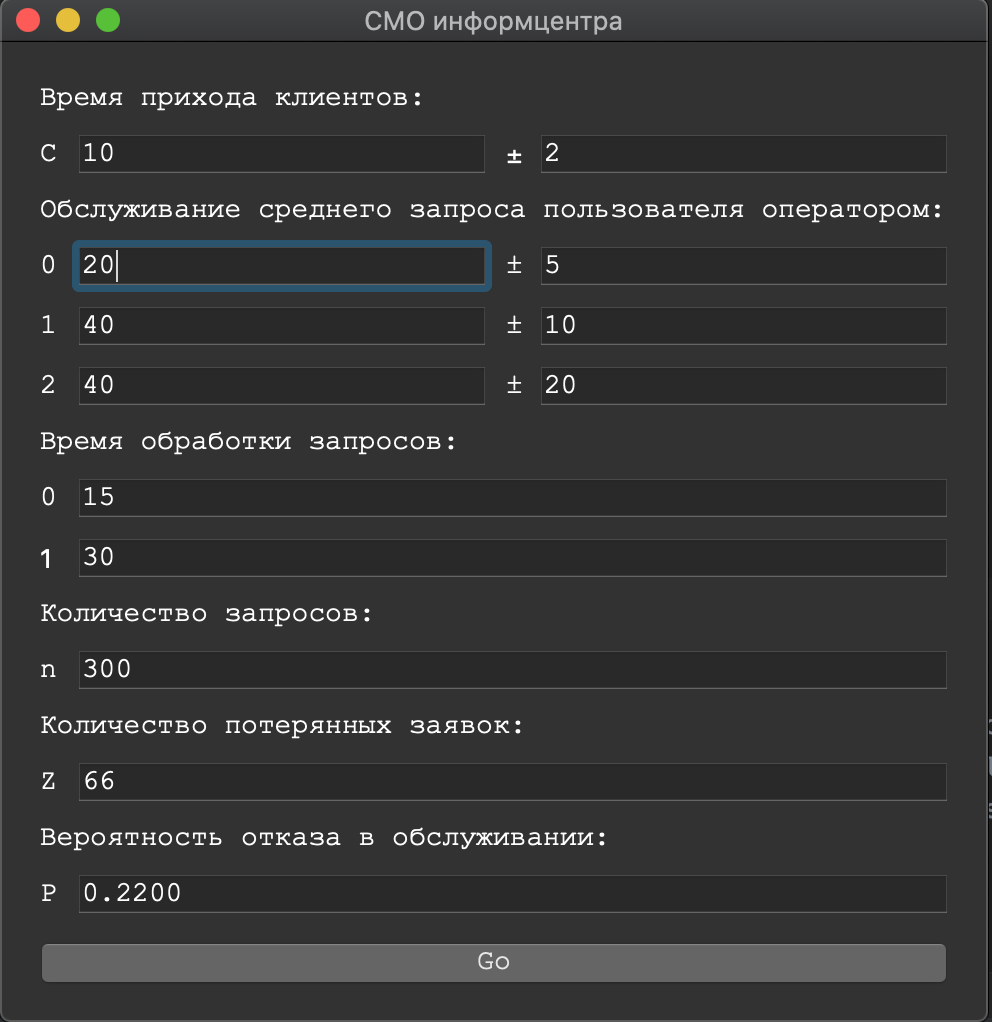
\includegraphics[width=\textwidth]{1.png}
		\end{minipage}
		\begin{minipage}[b]{0.32\textwidth}
			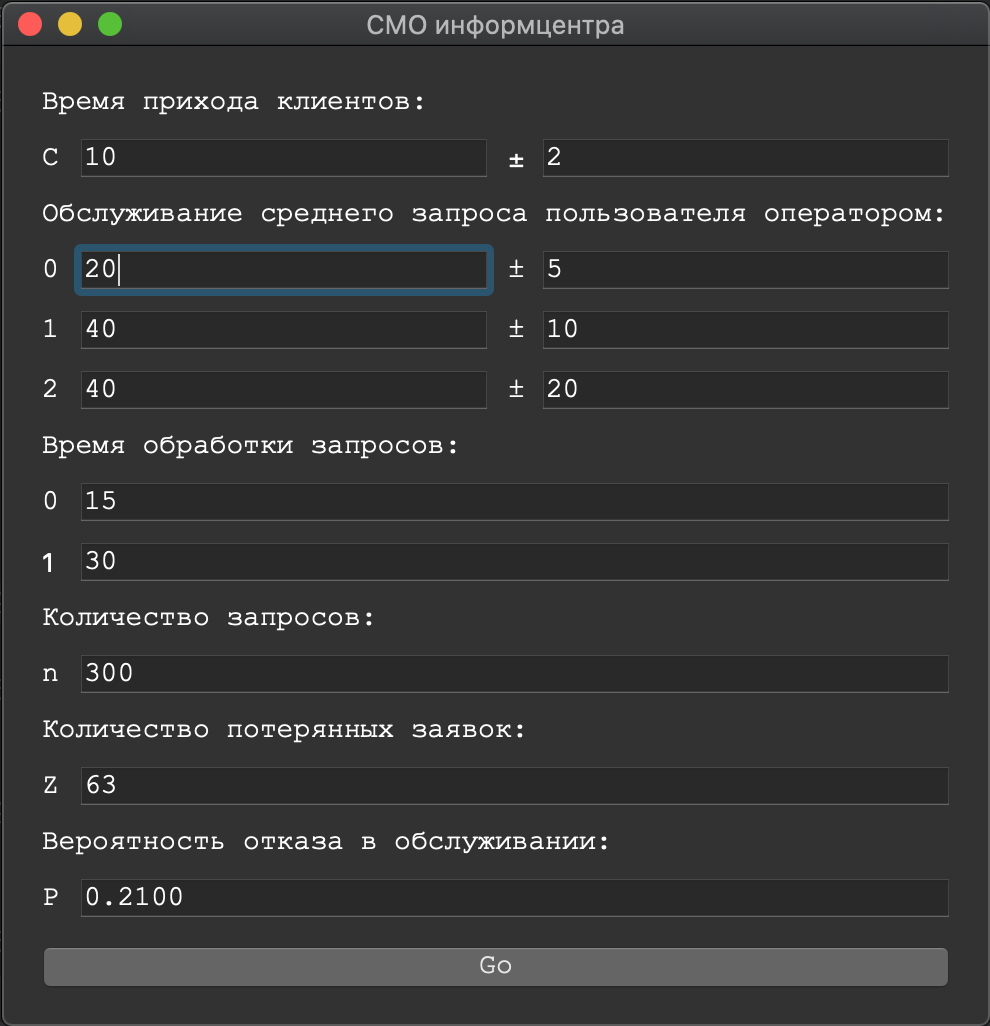
\includegraphics[width=\textwidth]{2.png}
		\end{minipage}
		\begin{minipage}[b]{0.32\textwidth}
			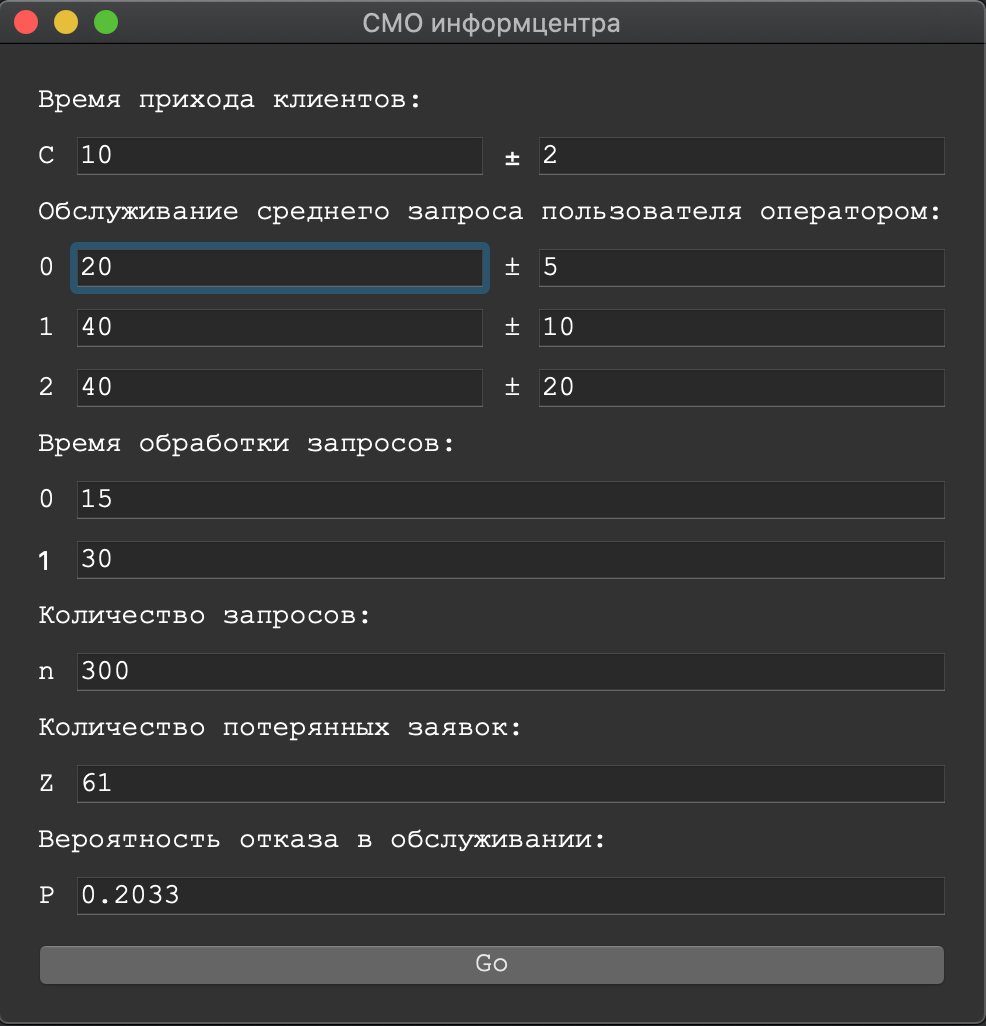
\includegraphics[width=\textwidth]{3.png}
		\end{minipage}
		\center{СМО информцентра}
		\label{ris:smo}
	\end{figure}
	
	\section*{Вывод}
	
	В результате проделанной работы была проведена формализация задачи, на основе чего была разработана программа, реализующая поставленную задачу.
	Программа позволяла определить количество потерянных заявок и вероятность отказа в обслуживании.
	
\end{document}